\subsection{PIMS Login Module}
This module is responsible for allowing a user to login into and Logout out of Pentec Patient Information Management System. A user should login with the credentials they were assigned upon registration. If the user is not assigned a user name then an exception is thrown and the user is redirected to the login page. \par 

To avoid "Spambots", a reCAPTCHA challenge is used. 

\subsubsection{Scope}
The scope is shown in the use case diagram below: \par
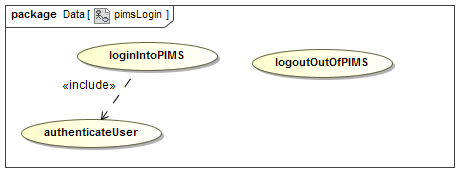
\includegraphics[width=0.75\linewidth]{./Graphics/pimsLogin/pimsLogin}

\subsubsection{Use cases}
\begin{description}
	\item{\textbf{loginToPIMS -- priority: critical}}\hfill
	This use case is to cater for the logging in of user into the system. It entails the authentication of each user as well as their authorization, which is based on their access rights.
		\begin{figure}[h!]
			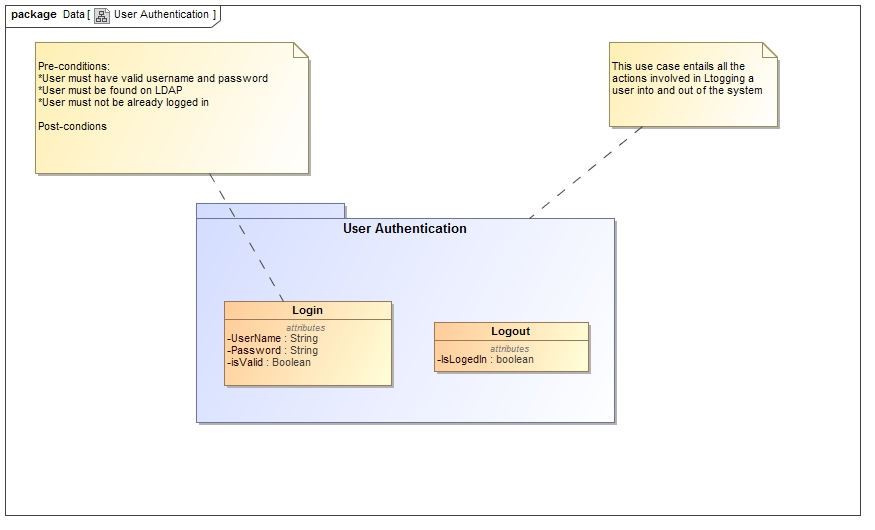
\includegraphics[width=0.7\linewidth]{./Graphics/Login}
		\end{figure}
	\item{\textbf{logoutOfPIMS -- priority: critical}}\hfill
	This use case logs a user out of the system by destroying the session. The user will not be allowed access unless they log back in.
		\begin{figure}[h!]
			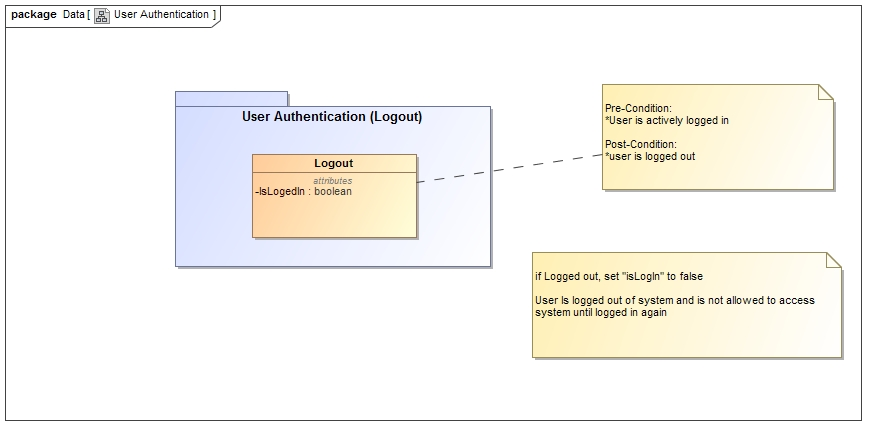
\includegraphics[width=0.7\linewidth]{./Graphics/Logout}
		\end{figure}
\end{description}
